\subsection{Representación gráfica del equipo}

Como se indicó anteriormente, la columna diseñada consta de 21 platos y la alimentación se introduce en el plato número 12. En la figura~\ref{fig:columna} se muestra esquemáticamente la configuración de la columna:

\begin{figure}[ht]
    \centering
    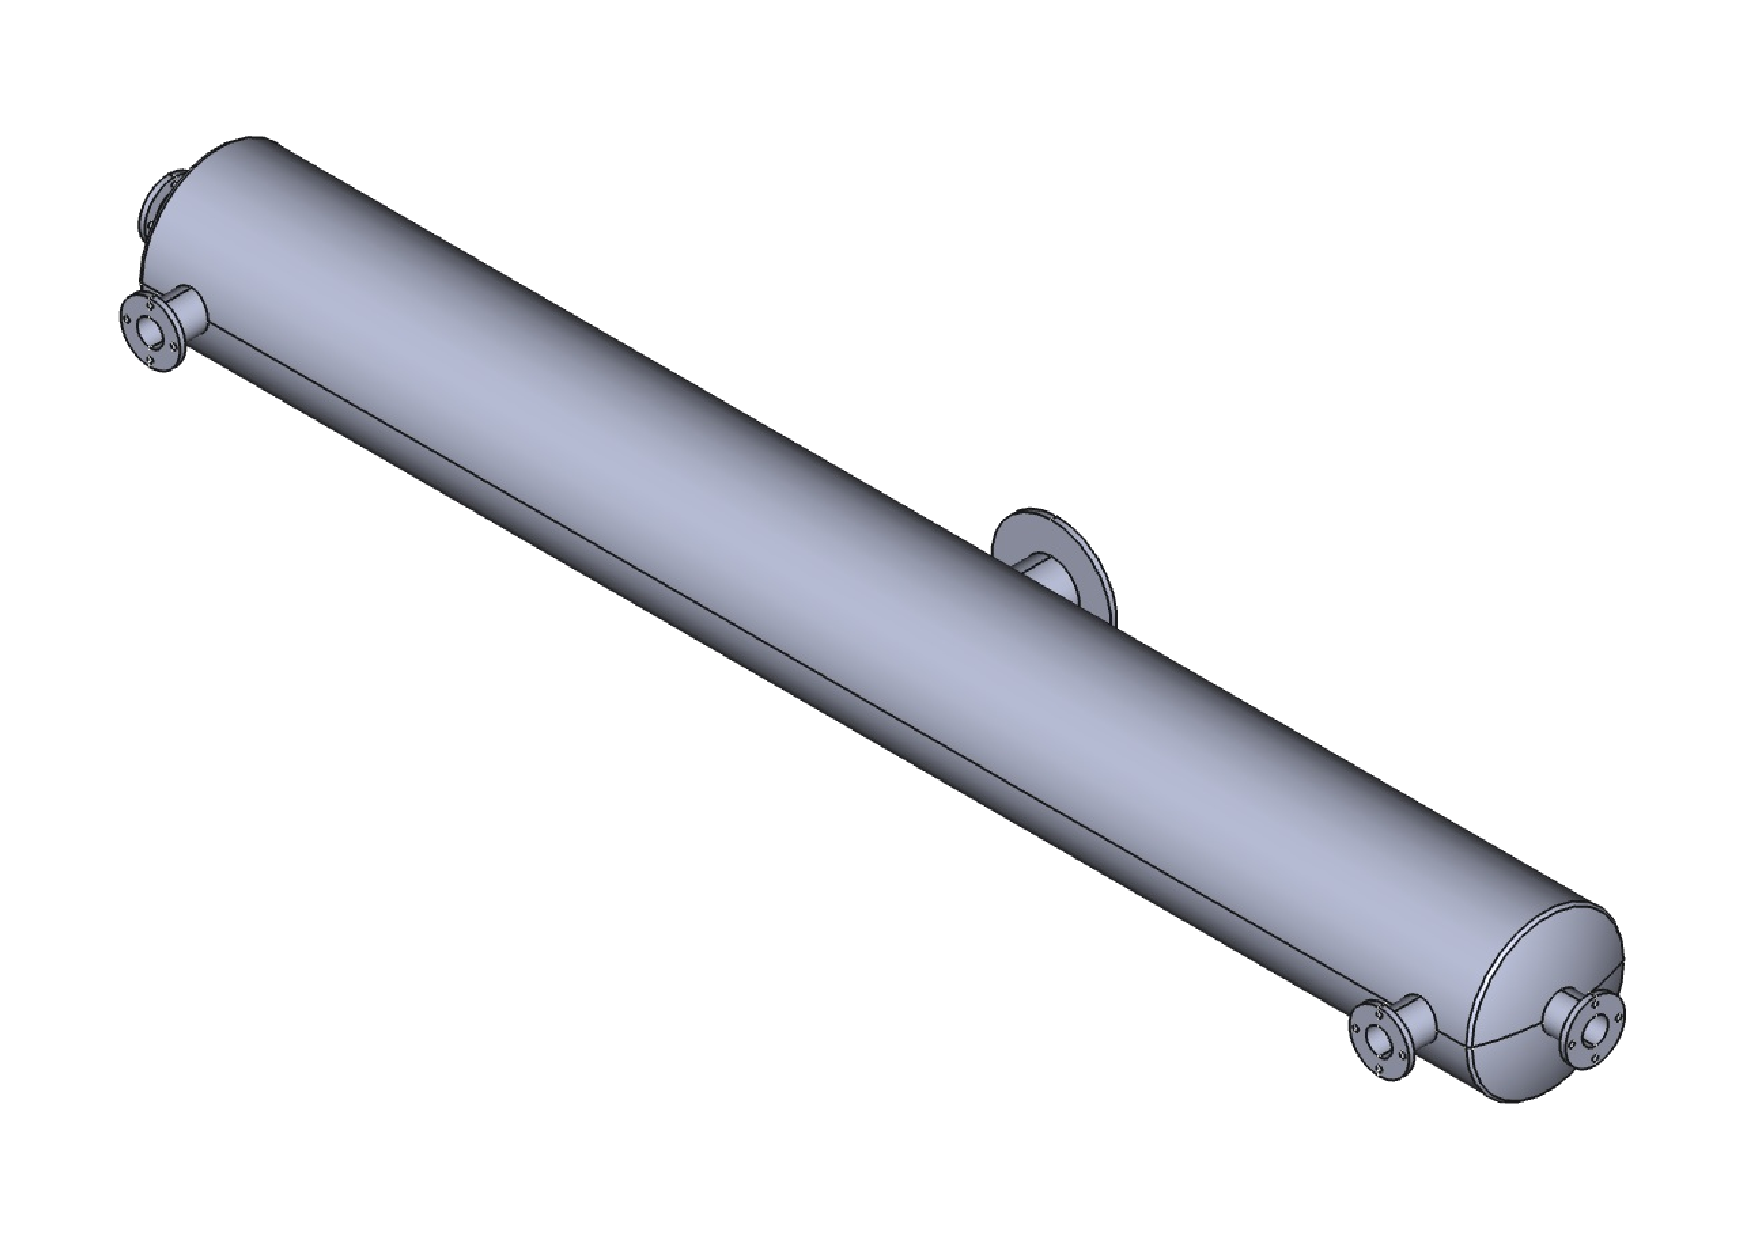
\includegraphics[width=1\linewidth]{../../desings/columna.pdf}
    \caption{Columna de destilación multicomponente}
    \label{fig:columna}
\end{figure}

Para los fines de la simulación, el condensador y el rehervidor se han considerado como platos (aunque en la realidad no lo son). Por este motivo, no se ha diseñado el condensador ni el rehervidor, ya que no forman parte del equipo principal (la columna).

\newpage
\vspace*{\fill}
Cada uno de los platos interiores de la columna corresponde a un plato perforado. Estos platos están dispuestos de tal manera que el líquido acumulado en la parte superior fluye hacia el plato inferior, mientras que el vapor ascendente atraviesa las perforaciones para alcanzar el plato superior. El diseño de los platos perforados se ilustra en la figura~\ref{fig:plato}:

\begin{figure}[ht]
    \centering
    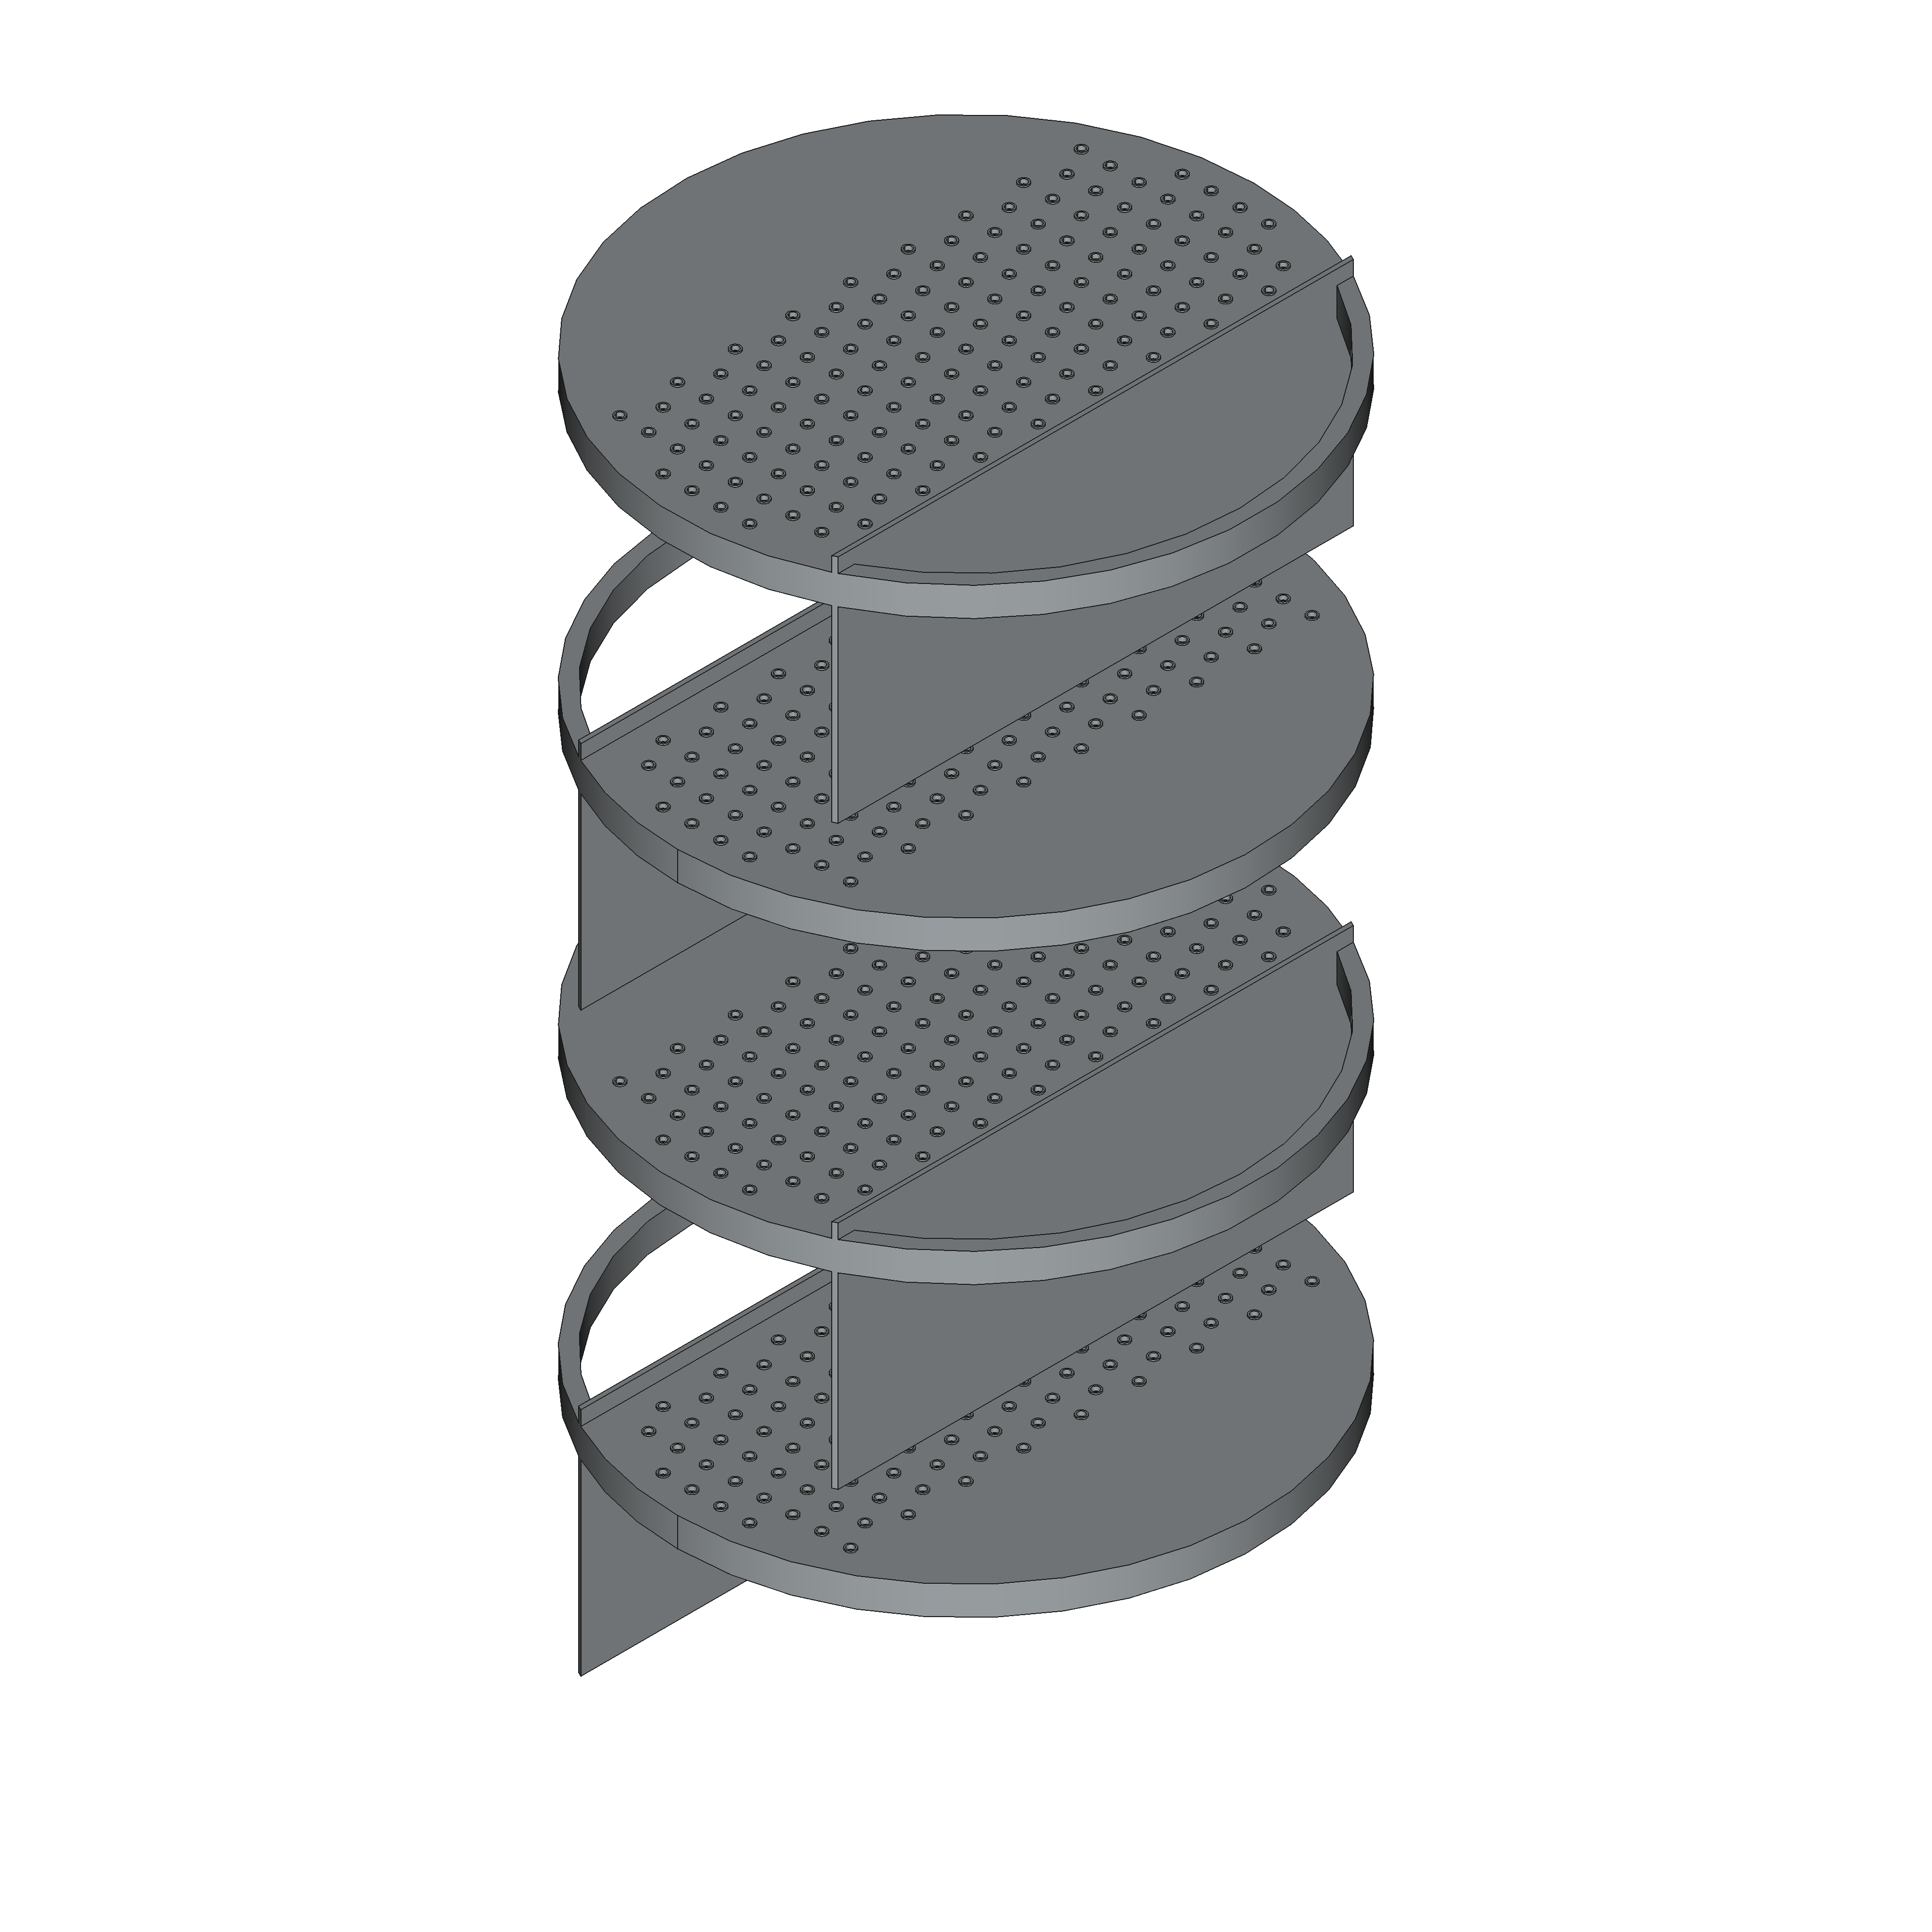
\includegraphics[width=1\linewidth]{../../desings/platos.png}
    \caption{Platos perforados para destilación multicomponente}
    \label{fig:plato}
\end{figure}
\vspace*{\fill}
